\documentclass[11pt]{article}
\usepackage[margin=1in]{geometry}
\usepackage{amsmath,amssymb}
\usepackage{booktabs}
\usepackage{tabularx}
\usepackage{longtable}
\usepackage{array}
\usepackage[round]{natbib}
\usepackage{xcolor}
\usepackage{tikz}
\usetikzlibrary{automata,positioning,arrows.meta,calc}
\usepackage{hyperref}
\usepackage{enumitem}
\setlist{nosep,leftmargin=*}
\hypersetup{colorlinks=true,linkcolor=blue!50!black,urlcolor=blue!50!black,citecolor=blue!50!black}
\newcolumntype{R}{>{\raggedleft\arraybackslash}X}
\newcommand{\SMB}{\textsc{smb}}
\newcommand{\HML}{\textsc{hml}}
\newcommand{\MOM}{\textsc{mom}}
\usepackage{xurl}
\newcommand{\doi}[1]{\href{https://doi.org/#1}{\nolinkurl{doi:#1}}}
\setlength{\emergencystretch}{2em}

\title{STA348 Term Project: Factor-Leadership Hidden Markov Model\\[4pt]\large Build Log --- Methods, Results and Return Tests}
\author{Richard}
\date{October 2026}

\begin{document}
\maketitle

\begin{abstract}
\noindent We model ``which equity factor is currently favoured'' as a hidden Markov chain over three states (\SMB, \HML, \MOM), observed through the factor that tops each period. The model is trained by Baum--Welch on the first half of the Ken French sample (1927--1976) and evaluated walk-forward on the second half (1976--2026), both on next-period prediction and on the returns earned by holding rules built on it. At monthly frequency the model finds clean, persistent regimes (expected durations of 7--10 months) whose labels survive every refit. Out of sample, however, it predicts the top factor no better than the raw transition matrix of observed tops (42.2\% vs 41.9\% hit rate; exact McNemar $p=0.90$), and no rule built on it beats an equal-weight factor portfolio on a risk-adjusted basis (best: probability tilt, Sharpe 0.63 vs 0.60; 95\% block-bootstrap interval for the difference $[-0.05,+0.12]$). Leadership regimes are real descriptively but carry no exploitable predictive content in this design.
\end{abstract}

\tableofcontents
\newpage

%==========================================================================
\section{Research question and scope}

\textbf{Question.} Is there a persistent underlying state in which one equity factor is favoured, and does knowing the current state help predict the next one, to the point of informing a smart-beta factor tilt?

\textbf{Approach.} A discrete hidden Markov model (HMM) with hidden states ``factor $k$ is favoured'' and observations ``factor $k$ topped this period''. The hidden layer is motivated by noise: the factor with the best return in a single period is partly luck, so treating it as the true state would overstate switching.

\textbf{Related work.} Regime-switching models have a long history in economics and finance \citep{hamilton1989,ang2012}. HMM regime identification on index returns is illustrated by \citet{yuan2016}. The closest applications to factor investing condition factor choice on market regimes \citep{wang2020}, identify regimes per factor \citep{shu2024}, or allocate across smart-beta strategies by regime \citep{fons2021}; none uses factor leadership itself as the hidden state.

\textbf{Scope of this log.} Version~1 of the model as specified in the design document \emph{Sta348 Model}, the data and engineering decisions made while building it, all results produced to date, and the return-testing procedure. Everything was implemented in \texttt{sta348\_hmm\_v1.py} (Python, \texttt{hmmlearn} 0.3.3 for Baum--Welch and Viterbi, \citealp{hmmlearn}; forward filtering hand-coded). Citation keys used in this log are listed in Appendix~\ref{sec:citemap}.

%==========================================================================
\section{Build timeline}

\begin{longtable}{@{}p{2.2cm}p{12.8cm}@{}}
\toprule
Step & Decision or outcome \\
\midrule
\endhead
Topic & Diamond--Dybvig bank-run chain rejected (transition probabilities would be assumed, not estimated). Factor leadership chosen: data-driven and fits the course toolkit. \\
Framing & Observable chain on the weekly top factor proposed first; moved to an HMM so that the hidden state is the favoured factor and the weekly top is a noisy reading of it. \\
Emissions & Continuous 4-vector emissions (multivariate normal) considered; replaced by the discrete encoding $o_t=\arg\max_k f_{k,t}$, which keeps the textbook machinery \citep[App.~A]{jurafsky_slp3} and a $3\times3$ emission matrix. \\
State set & Market excess return (RMRF) dropped from the state set: it is not a long--short spread, is far more volatile, and would make ``market-favoured'' mean ``the market rose''. States: \SMB, \HML, \MOM. \\
Naming & ``Soft naming'' adopted: Baum--Welch starts from emission rows tilted toward each state's own factor; names are checked afterwards by lift. \\
Design review & Corrections to the design document: $\pi$ uniform is $1/3$ (not $1/4$) with three states; rows of $B$ are states; \HML{} is value minus growth (not a ``growth premium''); the Carhart regression on page~1 is not used by the HMM. \\
v1 code & Implementation of training, Viterbi, forward filtering, walk-forward refit and benchmarks. Estimator verified on simulated data (Section~\ref{sec:sim}). \\
Pilot data & S\&P DJI index levels supplied. First set: momentum index covered one year only (53 common weeks; fit degenerate). Second set (10 years): pipeline works but states track market direction (Section~\ref{sec:pilot}). Abandoned for Ken French data. \\
Weekly run & French weekly 3-factor file plus daily momentum, compounded into French's own weeks; 5{,}212 weeks (Section~\ref{sec:weekly}). \\
Monthly run & French monthly files; returns test added (Sections~\ref{sec:monthly}--\ref{sec:returns}). \\
Diagnostics & Hit-rate comparison against the raw transition matrix; full-sample Viterbi encoding (Section~\ref{sec:viterbi}). \\
Start check & Starting $A$ counted from data compared with the assumed $A^{(0)}$; the assumed start kept (Section~\ref{sec:initrobust}). \\
TA feedback & Four validation extensions requested (cross-validation of the split, split-location sensitivity, randomised $A^{(0)}$, standard errors and a yearly block bootstrap). Specified in Section~\ref{sec:tafeedback}; \textbf{not yet implemented}. Cross-validation (Item~1) put on hold as covered by Items~2 and~4. \\
\bottomrule
\end{longtable}

%==========================================================================
\section{Data}

\subsection{Sources}
\begin{itemize}
\item \sloppy\textbf{Fama--French factors} (Ken French Data Library, \citealp{french_library}; CRSP database vintage 202609): monthly \texttt{F-F\_Research\_Data\_Factors} (\SMB, \HML), weekly \texttt{F-F\_Research\_Data\_Factors\_weekly}, monthly \texttt{F-F\_Momentum\_Factor} and daily \texttt{F-F\_Momentum\_Factor\_daily} (\MOM). Values are percent returns; converted to decimals.
\item \textbf{Pilot only:} S\&P DJI ``Performance Graph'' exports (S\&P 500 Momentum, S\&P 500 Value, S\&P 500/S\&P SmallCap 600 130/30), daily index levels 2016--2026.
\end{itemize}

\subsection{Factor definitions}
\SMB{} and \HML{} are built from six value-weighted portfolios formed each June from independent NYSE-breakpoint sorts on size (median) and book-to-market (30th/70th percentiles), following \citet{fama1993}:
\begin{align*}
\SMB_t &= \tfrac13(S/L+S/M+S/H)_t-\tfrac13(B/L+B/M+B/H)_t,\\
\HML_t &= \tfrac12(S/H+B/H)_t-\tfrac12(S/L+B/L)_t .
\end{align*}
\MOM{} (French version, not the PR1YR factor of \citealp{carhart1997}; the underlying momentum effect is documented by \citealp{jegadeesh1993}) is the average of the two high prior-return portfolios minus the two low prior-return portfolios from a $2\times3$ size by prior-return sort (prior return from month $-12$ to $-2$ in the monthly file; day $-250$ to $-21$ in the daily file). All three are zero-investment long--short returns.

\subsection{Frequency alignment}
\begin{itemize}
\item \textbf{Monthly:} the two monthly files are joined on month; the annual blocks appended to the files are skipped. Sample: January 1927 (first momentum month) to September 2026, $T=1{,}197$ months.
\item \textbf{Weekly:} French publishes no weekly momentum. Daily momentum is compounded into French's own weeks: day $d$ is assigned to the first weekly date $\ge d$, and $r^{\text{week}}=\prod(1+r^{\text{day}})-1$. A leading partial week is dropped. Sample: 6 November 1926 to 25 September 2026, $T=5{,}212$ weeks.
\end{itemize}

\subsection{Observation encoding}
\[
o_t=\arg\max_{k\in\{\SMB,\HML,\MOM\}} f_{k,t}\in\{0,1,2\},
\]
where $f_{k,t}$ is the return of factor $k$ in period $t$ (week or month), in decimals, taken from the Ken French files: $f_{\textsc{smb},t}=\SMB_t$, $f_{\textsc{hml},t}=\HML_t$, $f_{\textsc{mom},t}=\MOM_t$. The observation $o_t$ is the factor with the highest return that period, coded $0=\SMB$, $1=\HML$, $2=\MOM$. Example: in January 1927, $f_{\textsc{smb}}=-0.0047$, $f_{\textsc{hml}}=0.0476$, $f_{\textsc{mom}}=0.0057$, so $o_t=1$ (\HML).

Optional volatility scaling replaces $f_{k,t}$ by $\tilde f_{k,t}=f_{k,t}/\hat\sigma_{k,t-1}$ before the argmax, where $\hat\sigma_{k,t-1}$ is factor $k$'s standard deviation over the previous 52 weeks or 36 months (lagged one period so no future data enters). It is off by default (not in the design document); results with it are reported where informative.

%==========================================================================
\section{Model}

\subsection{Specification}
An HMM $\lambda=(A,B,\pi)$ \citep{rabiner1989,zucchini2016}, in the notation of \citet[App.~A]{jurafsky_slp3}, with
\begin{itemize}
\item hidden states $Q=\{q_1,q_2,q_3\}=\{\SMB,\HML,\MOM\}$, read as ``factor $k$ is currently favoured'';
\item transition matrix $A$, $a_{ij}=P(q_{t+1}=j\mid q_t=i)$;
\item emission matrix $B$, $b_j(k)=P(o_t=k\mid q_t=j)$, rows indexed by state;
\item initial distribution $\pi$.
\end{itemize}
Assumptions: first-order Markov property $P(q_t\mid q_{1:t-1})=P(q_t\mid q_{t-1})$ and output independence $P(o_t\mid q_{1:T},o_{-t})=P(o_t\mid q_t)$.

\subsection{Initial distribution}
$\pi$ is fixed at $(1/3,1/3,1/3)$ and not re-estimated. With a single long sequence, $\pi$ is informed by one observation, EM drives it to a corner, and it affects only the first few periods. (Option \texttt{--pi train} fixes it at the training top-factor frequencies instead.)

\subsection{Learning: Baum--Welch with soft naming}
\textbf{E-step} (scaled to avoid underflow, as in \citealp{rabiner1989}). Forward: $\alpha_1(j)=\pi_j b_j(o_1)$, $\alpha_t(j)=\big[\sum_i\alpha_{t-1}(i)a_{ij}\big]b_j(o_t)$. Backward: $\beta_T(i)=1$, $\beta_t(i)=\sum_j a_{ij}b_j(o_{t+1})\beta_{t+1}(j)$. Then
\[
\gamma_t(j)=\frac{\alpha_t(j)\beta_t(j)}{P(O\mid\lambda)},\qquad
\xi_t(i,j)=\frac{\alpha_t(i)a_{ij}b_j(o_{t+1})\beta_{t+1}(j)}{P(O\mid\lambda)}.
\]
\textbf{M-step.}
\[
\hat a_{ij}=\frac{\sum_{t=1}^{T-1}\xi_t(i,j)}{\sum_{t=1}^{T-1}\sum_k\xi_t(i,k)},\qquad
\hat b_j(k)=\frac{\sum_{t:\,o_t=k}\gamma_t(j)}{\sum_t\gamma_t(j)}.
\]
Iterate until the log-likelihood gain is below $10^{-6}$ (maximum 500 iterations). This is the Baum--Welch algorithm \citep{baum1970}, a special case of the EM algorithm \citep{dempster1977}.

\textbf{Starting values (soft-named start).} Baum--Welch needs a first guess $\lambda^{(0)}=(A^{(0)},B^{(0)},\pi)$ before the first forward--backward pass; see Section~\ref{sec:start} for the exact construction and the matrices used. Informed starting values are standard practice because EM converges to a local optimum that depends on where it starts \citep[p.~15]{jurafsky_slp3}, and because the likelihood does not identify which state is which (label switching; \citealp{stephens2000}).

\textbf{Restarts.} 20 runs: the soft start plus 19 jittered copies, built row by row for $A$ and $B$ as
\[
X\leftarrow\text{normalise}\big(0.8\,X^{(0)}+0.2\,\text{Dirichlet}(\mathbf 1)\big).
\] The run with the highest log-likelihood is kept; the share of runs that keep the soft names is reported. Multiple starting values are the usual guard against local optima in HMM estimation \citep{zucchini2016}.

\textbf{Name check (lift).} $L_{jk}=b_j(k)/\hat p_k$. State $j$ keeps its name if row $j$ of $L$ peaks on column $j$ and $L_{jj}>1$, i.e.\ factor $j$ tops more often than usual when state $j$ holds. Raw shares are not used because a frequently-topping factor can dominate every row. Lift is the association-rule measure of \citet{brin1997} (originally called ``interest''); the same ratio, under the name fold enrichment, is used to annotate fitted HMM states in genomics \citep{ernst2012,ernst2017}. Assigning names after fitting, rather than by constraints, follows the relabelling approach to label switching \citep{stephens2000}.

\subsection{Starting values: exact construction}\label{sec:start}
Throughout, rows and columns of every matrix are ordered (\SMB, \HML, \MOM); rows of $A$ are ``from'' states, rows of $B$ are hidden states and columns of $B$ are the observed top factor.

\textbf{Step 1: training frequencies.} Count the training periods in which each factor topped, $n_k=\#\{t\le T_{\text{train}}:o_t=k\}$, and set $\hat p_k=n_k/T_{\text{train}}$. Only training data are used.

\begin{center}
\begin{tabular}{lcccc}
\toprule
 & $n_{\textsc{smb}}$ & $n_{\textsc{hml}}$ & $n_{\textsc{mom}}$ & $\hat p=(\hat p_{\textsc{smb}},\hat p_{\textsc{hml}},\hat p_{\textsc{mom}})$ \\
\midrule
Monthly (598 months, Jan 1927 -- Oct 1976) & 146 & 174 & 278 & $(0.244,\ 0.291,\ 0.465)$ \\
Weekly (2{,}606 weeks, Nov 1926 -- Oct 1976) & 690 & 796 & 1{,}120 & $(0.265,\ 0.305,\ 0.430)$ \\
\bottomrule
\end{tabular}
\end{center}

\textbf{Step 2: emission start $B^{(0)}$ (data-built, tilted).} Each row starts at $\hat p$; the state's own factor is multiplied by a boost $c=2$ and the row is renormalised:
\[
b^{(0)}_j(k)=\frac{c^{\,\mathbf{1}[k=j]}\;\hat p_k}{1+(c-1)\hat p_j},
\qquad
B^{(0)}=
\begin{pmatrix}
\dfrac{2\hat p_1}{1+\hat p_1} & \dfrac{\hat p_2}{1+\hat p_1} & \dfrac{\hat p_3}{1+\hat p_1}\\[10pt]
\dfrac{\hat p_1}{1+\hat p_2} & \dfrac{2\hat p_2}{1+\hat p_2} & \dfrac{\hat p_3}{1+\hat p_2}\\[10pt]
\dfrac{\hat p_1}{1+\hat p_3} & \dfrac{\hat p_2}{1+\hat p_3} & \dfrac{2\hat p_3}{1+\hat p_3}
\end{pmatrix}.
\]
At the start, state $j$ makes its own factor $2/(1+\hat p_j)$ times as likely to top as usual (lift $1.37$--$1.61$) and every other factor $1/(1+\hat p_j)$ times as likely. No entry is zero, so Baum--Welch can move every entry.
\[
B^{(0)}_{\text{monthly}}=
\begin{pmatrix}
0.392 & 0.234 & 0.374\\
0.189 & 0.451 & 0.360\\
0.167 & 0.199 & 0.635
\end{pmatrix},
\qquad
B^{(0)}_{\text{weekly}}=
\begin{pmatrix}
0.419 & 0.242 & 0.340\\
0.203 & 0.468 & 0.329\\
0.185 & 0.214 & 0.601
\end{pmatrix}.
\]

\textbf{Step 3: transition start $A^{(0)}$ (assumed, symmetric).} A fixed persistence assumption, identical for every state and not computed from data, so that $A^{(0)}$ carries no information about which state is which (the naming comes from $B^{(0)}$ alone):
\[
a^{(0)}_{ij}=\begin{cases}s & i=j\\ \dfrac{1-s}{N-1} & i\ne j\end{cases},\quad s=0.8,\ N=3,
\qquad
A^{(0)}=
\begin{pmatrix}
0.8 & 0.1 & 0.1\\
0.1 & 0.8 & 0.1\\
0.1 & 0.1 & 0.8
\end{pmatrix}
\quad\text{(monthly and weekly).}
\]

\textbf{Step 4: initial distribution.} $\pi=(1/3,\,1/3,\,1/3)$, held fixed during training.

\textbf{Step 5: training.} All nine entries of $A$ and of $B$ are free; the starting values only decide where the iterations begin and therefore which state number ends up carrying which meaning.

\textbf{Alternative tested: data-built $A^{(0)}$.} As a robustness check (Section~\ref{sec:initrobust}), $A^{(0)}$ was instead counted from the observed top-factor sequence, with the same $B^{(0)}$. With $n_{ij}=\#\{t: o_t=i,\ o_{t+1}=j\}$ over training,
\[
a^{(0),\text{data}}_{ij}=\frac{n_{ij}+0.5}{\sum_k n_{ik}+1.5},
\qquad
N_{\text{monthly}}=
\begin{pmatrix}
42 & 36 & 67\\
33 & 64 & 77\\
71 & 73 & 134
\end{pmatrix},
\qquad
N_{\text{weekly}}=
\begin{pmatrix}
252 & 199 & 238\\
202 & 280 & 314\\
236 & 317 & 567
\end{pmatrix},
\]
\[
A^{(0),\text{data}}_{\text{monthly}}=
\begin{pmatrix}
0.290 & 0.249 & 0.461\\
0.191 & 0.368 & 0.442\\
0.256 & 0.263 & 0.481
\end{pmatrix},
\qquad
A^{(0),\text{data}}_{\text{weekly}}=
\begin{pmatrix}
0.366 & 0.289 & 0.345\\
0.254 & 0.352 & 0.394\\
0.211 & 0.283 & 0.506
\end{pmatrix}.
\]
This is the observable chain's transition matrix: weak persistence (diagonals 0.29--0.51) and every monthly row peaking on \MOM.

\subsection{Decoding and forecasting}
\textbf{Viterbi} \citep{viterbi1967} (Problem~2 in the classification of \citealp{rabiner1989}), used only to describe history: $v_t(j)=\max_i v_{t-1}(i)a_{ij}b_j(o_t)$ with back-pointers. Viterbi and smoothed probabilities use future observations, so they are never used in testing.

\textbf{Filtering} (Problem~1; the scaled forward recursion of \citealp{rabiner1989}, known in econometrics as the filter of \citealp{hamilton1989}), used for every forecast. With $\hat\alpha_t$ the normalised forward vector,
\[
P(q_{t+1}=j\mid o_{1:t})=\sum_i\hat\alpha_t(i)a_{ij},\qquad
P(o_{t+1}=k\mid o_{1:t})=\sum_j P(q_{t+1}=j\mid o_{1:t})\,b_j(k).
\]

\subsection{Validation design}
\begin{enumerate}
\item \textbf{Chronological split} 50/50: training = first half, test = second half. No test observation enters training (out-of-sample evaluation in time order; \citealp{tashman2000}).
\item \textbf{Walk-forward.} For each test period $t$: forecast $o_t$ from $o_{1:t-1}$, record, observe $o_t$, update $\hat\alpha$, and refit Baum--Welch on $o_{1:t}$ warm-started from the current $(A,B)$ (keeps labels fixed; one run, no restarts). Refit every period by default; \texttt{--refit-every 0} freezes the trained parameters. This is rolling-origin (walk-forward) evaluation \citep{tashman2000}.
\item \textbf{Prediction rules.} (a) design-document rule: the most likely next \emph{state}, compared with the actual top factor; (b) the most likely next \emph{top factor}, $\arg\max_k P(o_t=k\mid o_{1:t-1})$.
\item \textbf{Benchmarks} re-estimated on $o_{1:t-1}$ each period: the raw MLE transition matrix of observed tops, $\hat a^{\text{obs}}_{ij}\propto n_{ij}+0.5$ (observable chain); ``same as last period''; ``most frequent factor so far''.
\item \textbf{Metrics.} Hit rate with binomial standard error; average log score $\frac1n\sum_t\log P(o_t\mid o_{1:t-1})$, a strictly proper scoring rule \citep{gneiting2007}; paired log-score difference with standard error, in the spirit of \citet{diebold1995}; exact McNemar test on periods where two predictors disagree \citep{mcnemar1947}.
\end{enumerate}

\subsection{In-sample model checks}
BIC \citep{schwarz1978} comparison of a no-memory model (2 free parameters), the observable chain (8) and the HMM (12, $\pi$ fixed), with differences read on the evidence scale of \citet{kass1995}; a simulation check in the spirit of posterior predictive checks \citep{gelman1996} comparing the observed switching rate and repeat probabilities of the top factor with 300 sequences simulated from the fitted model.

%==========================================================================
\section{Return-testing procedure}\label{sec:returnsmethod}

Hit rate ignores magnitudes; the return test asks what following each rule would have earned. All decisions for period $t$ use data through $t-1$ only.

\textbf{State-conditional means.} With smoothed weights $\gamma_s(k)$ computed on data through the last refit,
\[
\mu_k=\frac{\sum_s\gamma_s(k)\,\mathbf r_s}{\sum_s\gamma_s(k)}\in\mathbb R^3,
\qquad
\mathbb E[\mathbf r_t\mid o_{1:t-1}]=\sum_k P(q_t=k\mid o_{1:t-1})\,\mu_k .
\]
Smoothing within the past window is not look-ahead; $\mu_k$ is re-estimated at each refit.

\textbf{Observable-chain conditional means.} $m_j=$ average of $\mathbf r_{s+1}$ over past $s$ with $o_s=j$; the forecast for $t$ is $m_{o_{t-1}}$.

\textbf{Rules} (weights $\mathbf w_t$ on the three factors):
\begin{center}
\begin{tabularx}{\textwidth}{@{}lX@{}}
\toprule
Rule & Weights \\
\midrule
HMM expected & all in $\arg\max_k \mathbb E[r_{k,t}\mid o_{1:t-1}]$ \\
HMM top & all in $\arg\max_k P(o_t=k\mid o_{1:t-1})$ \\
HMM tilt & $w_{k,t}=P(o_t=k\mid o_{1:t-1})$ \\
Chain expected & all in $\arg\max_k m_{o_{t-1},k}$ \\
Last winner & all in $o_{t-1}$ \\
Best so far & all in the factor with the highest average return to date \\
Equal weight & $1/3$ each (benchmark; the $1/N$ rule of \citealp{demiguel2009}) \\
\bottomrule
\end{tabularx}
\end{center}

\textbf{Metrics.} Portfolio return $r^p_t=\mathbf w_t^\top\mathbf r_t$. With $P=12$ (monthly) or 52 (weekly): annualised mean $P\bar r$, volatility $\sqrt P s$, Sharpe ratio $\sqrt P\,\bar r/s$ \citep{sharpe1994} (no risk-free rate: the factors are zero-cost returns), maximum drawdown of $\prod(1+r^p_t)$, and average weight traded $\sum_k|w_{k,t}-w_{k,t-1}|$. Net returns subtract 10 bp per unit traded (a full switch trades 2 units). Significance: paired $t$-statistic of the mean return difference versus equal weight, and a 12-month moving-block bootstrap \citep{kunsch1989} (2{,}000 draws) of the Sharpe difference versus equal weight, a simpler relative of the bootstrap Sharpe-ratio tests of \citet{ledoit2008}.

%==========================================================================
\section{Estimator verification on simulated data}\label{sec:sim}

3{,}000 periods were simulated from $a_{jj}=0.90$, $a_{ij}=0.05$, $b_j(j)=0.60$, $b_j(k)=0.20$, then passed through the full pipeline (1{,}500 training periods, refit every 4).
\begin{itemize}
\item All 20 restarts kept the soft names; recovered diagonals $\hat a_{jj}=(0.876,0.944,0.977)$ and $\hat b_j(j)=(0.688,0.507,0.559)$. Structure recovered; individual entries imprecise even at 1{,}500 periods.
\item Out of sample the HMM beat the observable chain where a true hidden structure exists: hit rate 46.5\% vs 43.1\%, log-score difference $+0.022$ (s.e.\ 0.006).
\end{itemize}
The code therefore can detect a hidden-state advantage when one exists.

%==========================================================================
\section{Pilot: S\&P DJI index data}\label{sec:pilot}

\textbf{First set.} The momentum export covered one year, leaving 53 common weeks (26 for training). The fit was degenerate (names failed; one absorbing state). Not interpretable.

\textbf{Ten-year set} (526 weeks, Oct 2016--Oct 2026). Names failed (rows peaked on \HML, \HML, \SMB; 45\% of starts kept them; names drifted in all 262 refits). Out of sample: HMM top-factor rule 42.2\%, raw matrix 40.7\%, most frequent 41.8\%; log-score difference $+0.002$ (s.e.\ 0.010).

\textbf{Diagnosis.} The indices are long-only and highly correlated (weekly $\rho=0.75$--$0.89$), so the argmax mostly reflects market direction:
\begin{center}
\begin{tabular}{lccc}
\toprule
 & Value tops & Momentum tops & 130/30 tops \\
\midrule
Up weeks & 27\% & 50\% & 23\% \\
Down weeks & 43\% & 31\% & 26\% \\
\bottomrule
\end{tabular}
\end{center}
Subtracting a market return does not help, since it does not change the argmax. The 130/30 index is also not a size factor. The pilot was abandoned in favour of the long--short French factors.

%==========================================================================
\section{Results: weekly French data}\label{sec:weekly}

Training 6 Nov 1926 -- 15 Oct 1976 (2{,}606 weeks); test to 25 Sep 2026 (2{,}606 weeks). Training top shares: \SMB{} 26.5\%, \HML{} 30.5\%, \MOM{} 43.0\%.

\subsection{Trained parameters}
Best log-likelihood $-2{,}761.80$; 90\% of restarts kept the soft names; no name drift in 2{,}605 refits.
\begin{center}
\begin{tabular}{l ccc c ccc c ccc}
\toprule
 & \multicolumn{3}{c}{$A$ (to)} && \multicolumn{3}{c}{$B$ (tops)} && \multicolumn{3}{c}{Lift} \\
\cmidrule{2-4}\cmidrule{6-8}\cmidrule{10-12}
From & \SMB & \HML & \MOM && \SMB & \HML & \MOM && \SMB & \HML & \MOM \\
\midrule
\SMB & .732 & .018 & .250 && .485 & .339 & .176 && 1.83 & 1.11 & 0.41 \\
\HML & .193 & .807 & .000 && .000 & .560 & .440 && 0.00 & 1.83 & 1.02 \\
\MOM & .326 & .046 & .628 && .037 & .159 & .804 && 0.14 & 0.52 & 1.87 \\
\bottomrule
\end{tabular}
\end{center}
Expected durations $1/(1-a_{jj})$: 3.7, 5.2, 2.7 weeks. Stationary distribution: (0.520, 0.132, 0.349). Training Viterbi run lengths: 5.5, 12.2, 3.9 weeks, versus 1.6, 1.5, 2.0 weeks for the raw top factor.

\subsection{Model checks}
\begin{center}
\begin{tabular}{lrrr}
\toprule
Model (training) & Log-lik. & Params & BIC \\
\midrule
No memory & $-2{,}806.8$ & 2 & 5{,}629.3 \\
Observable chain & $-2{,}769.7$ & 8 & \textbf{5{,}602.3} \\
HMM & $-2{,}761.8$ & 12 & 5{,}618.0 \\
\bottomrule
\end{tabular}
\end{center}
Weekly leadership has memory (both chains beat no-memory), but the hidden layer does not justify its parameters. Posterior predictive check passed: observed switching rate 0.578 vs simulated 95\% range [0.564, 0.606]; repeat probabilities within range for all three factors.

\subsection{Out-of-sample prediction}
\begin{center}
\begin{tabular}{lccc}
\toprule
Predictor (2{,}606 test weeks) & Hit rate & s.e. & Log score \\
\midrule
HMM, most likely top factor & 40.1\% & 1.0 & $-1.087$ \\
HMM, most likely state (design-doc rule) & 33.4\% & 0.9 & $-1.087$ \\
Raw transition matrix & 39.6\% & 1.0 & $-1.090$ \\
Same as last week & 37.6\% & 0.9 & --- \\
Most frequent so far & 40.1\% & 1.0 & $-1.090$ \\
\bottomrule
\end{tabular}
\end{center}
Log-score difference HMM minus raw matrix: $+0.0040$ (s.e.\ 0.0022). Frozen parameters: $+0.0000$ (s.e.\ 0.0021); volatility-scaled: $+0.0039$ (s.e.\ 0.0026). The two predictors agree in 79.6\% of weeks; of the 531 disagreements the HMM is right 199 times, the raw matrix 186, neither 146 (exact McNemar $p=0.54$). By decade the HMM leads in the 1980s--2000s and trails in the 2010s.

%==========================================================================
\section{Results: monthly French data (main specification)}\label{sec:monthly}

Training Jan 1927 -- Oct 1976 (598 months); test Nov 1976 -- Sep 2026 (599 months). Training top shares: \SMB{} 24.4\%, \HML{} 29.1\%, \MOM{} 46.5\%; test: 28.0\%, 30.1\%, 41.9\%.

\subsection{Trained automaton}
Best log-likelihood $-620.93$; 95\% of restarts kept the soft names; names held in all 598 walk-forward refits. Starting from $A^{(0)}$ and $B^{(0)}_{\text{monthly}}$ of Section~\ref{sec:start}, Baum--Welch converged to (rows and columns ordered \SMB, \HML, \MOM):
\[
\hat A_{\text{monthly}}=
\begin{pmatrix}
0.864 & 0.067 & 0.069\\
0.101 & 0.899 & 0.000\\
0.092 & 0.052 & 0.857
\end{pmatrix},
\qquad
\hat B_{\text{monthly}}=
\begin{pmatrix}
0.398 & 0.107 & 0.494\\
0.208 & 0.472 & 0.320\\
0.000 & 0.330 & 0.670
\end{pmatrix}.
\]
Change from the start: the diagonal of $A$ rose from 0.8 to 0.86--0.90; in $B$ the \SMB{} state's \HML{} entry fell from 0.234 to 0.107 and its \MOM{} entry rose from 0.374 to 0.494, while the \HML{} row moved little. Figure~\ref{fig:automaton} shows the estimated machine.

\begin{figure}[h]
\centering
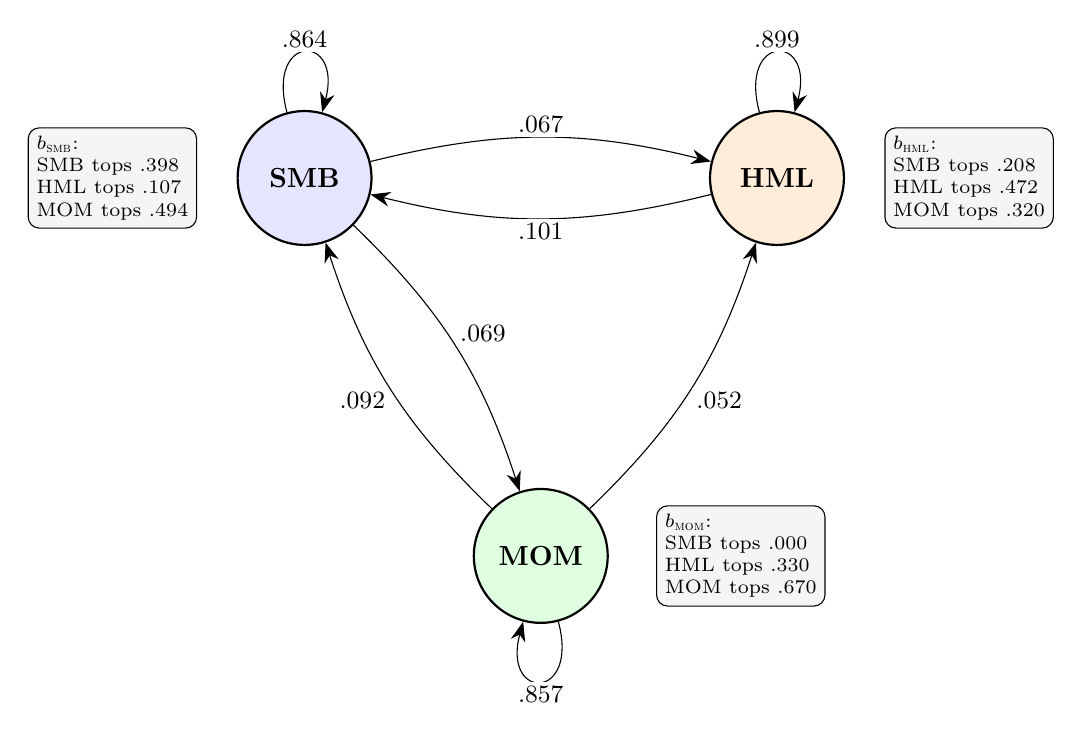
\begin{tikzpicture}[
  >={Stealth[length=2.5mm]}, node distance=4.6cm, auto,
  every state/.style={draw, thick, minimum size=1.7cm, font=\bfseries},
  lbl/.style={font=\small, fill=white, inner sep=1.5pt},
  em/.style={draw, rounded corners, font=\scriptsize, align=left, fill=gray!8, inner sep=3pt}]
  \node[state, fill=blue!10]  (S) at (0,0)       {SMB};
  \node[state, fill=orange!15] (H) at (6,0)      {HML};
  \node[state, fill=green!12] (M) at (3,-4.8)    {MOM};
  % self loops
  \path[->] (S) edge[loop above, looseness=6] node[lbl] {.864} (S);
  \path[->] (H) edge[loop above, looseness=6] node[lbl] {.899} (H);
  \path[->] (M) edge[loop below, looseness=6] node[lbl] {.857} (M);
  % transitions (HML -> MOM estimated at 0.000, omitted)
  \path[->] (S) edge[bend left=14] node[lbl] {.067} (H);
  \path[->] (H) edge[bend left=14] node[lbl] {.101} (S);
  \path[->] (S) edge[bend left=14] node[lbl] {.069} (M);
  \path[->] (M) edge[bend left=14] node[lbl] {.092} (S);
  \path[->] (M) edge[bend right=14, swap] node[lbl] {.052} (H);
  % emissions
  \node[em, left=0.5cm of S] {$b_{\textsc{smb}}$:\\ SMB tops .398\\ HML tops .107\\ MOM tops .494};
  \node[em, right=0.5cm of H] {$b_{\textsc{hml}}$:\\ SMB tops .208\\ HML tops .472\\ MOM tops .320};
  \node[em, right=0.6cm of M] {$b_{\textsc{mom}}$:\\ SMB tops .000\\ HML tops .330\\ MOM tops .670};
\end{tikzpicture}
\caption{Estimated monthly automaton, training window 1927--1976. Arrows carry $a_{ij}$; boxes carry the emission rows $b_j(\cdot)$. The \HML$\to$\MOM{} transition and the \MOM-state emission of an \SMB{} top were estimated at zero (EM boundary solutions). $\pi=(1/3,1/3,1/3)$, fixed.}
\label{fig:automaton}
\end{figure}

\begin{center}
\begin{tabular}{l ccc c ccc c c c}
\toprule
 & \multicolumn{3}{c}{Lift $b_j(k)/\hat p_k$} && \multicolumn{3}{c}{Mean return in state (\%/mo)} && Exp.\ dur. & Stationary \\
\cmidrule{2-4}\cmidrule{6-8}
State & \SMB & \HML & \MOM && \SMB & \HML & \MOM && (months) & share \\
\midrule
\SMB & \textbf{1.63} & 0.37 & 1.06 && 0.59 & $-0.27$ & 0.73 && 7.4 & 0.418 \\
\HML & 0.85 & \textbf{1.62} & 0.69 && 0.30 & 1.30 & 0.22 && 9.9 & 0.382 \\
\MOM & 0.00 & 1.13 & \textbf{1.44} && $-0.72$ & 0.46 & 1.29 && 7.0 & 0.200 \\
\bottomrule
\end{tabular}
\end{center}
Mean returns use smoothed weights over the training window. Raw transition matrix of observed tops (training): every row peaks on \MOM{} (0.461, 0.442, 0.481). Training Viterbi run lengths: 16.7, 28.3, 15.8 months versus 1.4, 1.6, 1.9 for the raw top factor.

\subsection{Model checks}
\begin{center}
\begin{tabular}{lrrr}
\toprule
Model (training) & Log-lik. & Params & BIC \\
\midrule
No memory & $-633.6$ & 2 & \textbf{1{,}280.0} \\
Observable chain & $-629.1$ & 8 & 1{,}309.4 \\
HMM & $-620.9$ & 12 & 1{,}318.6 \\
\bottomrule
\end{tabular}
\end{center}
At monthly frequency BIC prefers the no-memory model: the HMM's likelihood gain does not cover its extra parameters. Posterior predictive check passed (switching rate 0.598 vs [0.538, 0.632]; repeat probabilities within range). Volatility scaling broke the names at monthly frequency (rows peaked on \SMB, \HML, \SMB; drift in all refits) and is not used.

\subsection{Out-of-sample prediction}
\begin{center}
\begin{tabular}{lccc}
\toprule
Predictor (599 test months) & Hit rate & s.e. & Log score \\
\midrule
HMM, most likely top factor & 42.2\% & 2.0 & $-1.089$ \\
HMM, most likely state (design-doc rule) & 32.4\% & 1.9 & $-1.089$ \\
Raw transition matrix & 41.9\% & 2.0 & $-1.084$ \\
Same as last month & 38.2\% & 2.0 & --- \\
Most frequent so far & 41.9\% & 2.0 & $-1.086$ \\
\bottomrule
\end{tabular}
\end{center}
Log-score difference HMM minus raw matrix: $-0.0058$ (s.e.\ 0.0047).

\textbf{Hit-rate diagnostics against the raw matrix.}
\begin{itemize}
\item The raw matrix predicts \MOM{} in all 599 months (every row peaks on \MOM), so it equals ``always the most frequent factor''. Its 41.9\% is the test share of \MOM{} tops.
\item The HMM predicts \MOM{} in 86.6\% of months and \HML{} in 13.4\%; it never predicts \SMB{} although \SMB{} topped in 28\% of months.
\item In the 80 disagreements (always HMM \HML{} vs raw \MOM): \HML{} topped 31 times, \MOM{} 29, \SMB{} 20. Exact McNemar $p=0.90$.
\item Conditional on last month's top factor the hit rates are near-identical (after \SMB: 42.9\% vs 42.9\%; \HML: 40.0\% vs 38.3\%; \MOM: 43.2\% vs 43.6\%). No decade shows a gap above 2.7 points.
\end{itemize}

%==========================================================================
\section{Results: return tests (monthly)}\label{sec:returns}

Procedure as in Section~\ref{sec:returnsmethod}; test window Nov 1976 -- Sep 2026, 599 months.

\begin{center}
\footnotesize
\setlength{\tabcolsep}{4pt}
\begin{tabular}{lrrrrrrr}
\toprule
Rule & Return & Vol & Sharpe & Max DD & Traded & Net Sharpe & $t$ vs EW \\
 & (\%/yr) & (\%/yr) & & (\%) & /month & & (mean) \\
\midrule
Equal weight (benchmark) & 3.74 & 6.18 & 0.604 & $-24.7$ & 0.00 & 0.604 & --- \\
HMM tilt ($w=P(\text{tops})$) & 4.56 & 7.30 & 0.625 & $-25.5$ & 0.10 & 0.608 & 2.53 \\
Chain expected & 8.47 & 13.40 & 0.632 & $-40.8$ & 0.76 & 0.564 & 2.97 \\
Last winner & 7.66 & 12.47 & 0.614 & $-39.9$ & 1.23 & 0.495 & 2.56 \\
HMM top & 7.54 & 14.64 & 0.515 & $-55.0$ & 0.32 & 0.489 & 2.30 \\
Best so far & 6.95 & 15.16 & 0.458 & $-57.8$ & 0.00 & 0.458 & 1.94 \\
HMM expected & 5.93 & 14.44 & 0.411 & $-64.1$ & 0.60 & 0.361 & 1.32 \\
\bottomrule
\end{tabular}
\end{center}

\textbf{Sharpe difference versus equal weight} (gross; 12-month block bootstrap, 2{,}000 draws):
\begin{center}
\begin{tabular}{lcc}
\toprule
Rule & $\Delta$ Sharpe & 95\% interval \\
\midrule
HMM tilt & $+0.021$ & [$-0.047$, $+0.120$] \\
Chain expected & $+0.028$ & [$-0.206$, $+0.278$] \\
Last winner & $+0.010$ & [$-0.202$, $+0.284$] \\
HMM top & $-0.089$ & [$-0.319$, $+0.182$] \\
Best so far & $-0.146$ & [$-0.370$, $+0.138$] \\
HMM expected & $-0.193$ & [$-0.407$, $+0.059$] \\
\bottomrule
\end{tabular}
\end{center}

\textbf{Reading.}
\begin{itemize}
\item The positive $t$-statistics against equal weight compare \emph{mean} returns; single-factor rules earn more because they carry roughly twice the volatility. On Sharpe, no rule is distinguishable from equal weight.
\item The HMM tilt is the only HMM rule that does not lose to equal weight; its edge is 0.02 gross and under 0.01 after costs.
\item Switching on HMM expected returns is the worst rule (Sharpe 0.41, drawdown $-64\%$, much of it the 2009 momentum crash): the state means estimated in 1927--1976 did not persist.
\end{itemize}

%==========================================================================
\section{Robustness: assumed versus data-built starting $A$}\label{sec:initrobust}

\textbf{Method.} Training was repeated with two first guesses that differ only in $A^{(0)}$ (Section~\ref{sec:start}); everything else is identical: the same data-built $B^{(0)}$, $\pi$ fixed at $1/3$, 20 starts (the exact start plus 19 jittered copies, seed 348), at most 500 iterations, tolerance $10^{-6}$.
\begin{itemize}
\item \textbf{Version 1 (used):} $B^{(0)}$ from data, $A^{(0)}$ assumed ($0.8$ diagonal, $0.1$ elsewhere).
\item \textbf{Version 2:} $B^{(0)}$ from data, $A^{(0)}$ counted from data ($A^{(0),\text{data}}$).
\end{itemize}
To check whether two fitted models are the same up to a renumbering of states, all $3!=6$ permutations $\sigma$ were tried and the one minimising $\max|A_2[\sigma,\sigma]-A_1|+\max|B_2[\sigma,\cdot]-B_1|$ kept. For monthly data the walk-forward test (refit every 4 months) was also run for both versions.

\subsection{Monthly}
\begin{center}
\begin{tabular}{lcc}
\toprule
 & $A^{(0)}$ assumed & $A^{(0)}$ from data \\
\midrule
Log-likelihood from the exact start & $-621.54$ & $-620.93$ \\
Best log-likelihood over 20 starts & $-620.93$ & $-620.93$ \\
Starts keeping the soft names & 95\% & 40\% \\
Lift on own factor (\SMB, \HML, \MOM) & 1.63, 1.62, 1.44 & 0.85, 1.13, 1.06 \\
Names supported & Yes & No \\
Walk-forward hit rate / log score & 41.9\% / $-1.0888$ & 41.9\% / $-1.0888$ \\
Probability-tilt Sharpe (gross) & 0.624 & 0.624 \\
\bottomrule
\end{tabular}
\end{center}
Trained matrices of version 2, in its own state order (\SMB, \HML, \MOM):
\[
\hat A^{\text{data}}_{\text{monthly}}=
\begin{pmatrix}
0.899 & 0.000 & 0.101\\
0.051 & 0.857 & 0.092\\
0.068 & 0.068 & 0.864
\end{pmatrix},
\qquad
\hat B^{\text{data}}_{\text{monthly}}=
\begin{pmatrix}
0.208 & 0.472 & 0.320\\
0.000 & 0.330 & 0.670\\
0.398 & 0.107 & 0.494
\end{pmatrix}.
\]
Comparing with $\hat A_{\text{monthly}},\hat B_{\text{monthly}}$ in Section~\ref{sec:monthly}: version 2's ``\SMB'' state is version 1's \HML{} state, its ``\HML'' is \MOM{} and its ``\MOM'' is \SMB. After this renumbering the two fits agree to within 0.0006 ($A$) and 0.0002 ($B$). It is the same model with the labels rotated, which is why every out-of-sample number is identical: predictions do not depend on state names.

\subsection{Weekly}
\begin{center}
\begin{tabular}{lcc}
\toprule
 & $A^{(0)}$ assumed & $A^{(0)}$ from data \\
\midrule
Log-likelihood from the exact start & $-2{,}761.80$ & $-2{,}767.45$ \\
Best log-likelihood over 20 starts & $\mathbf{-2{,}761.80}$ & $-2{,}764.83$ \\
Starts keeping the soft names & 90\% & 95\% \\
Lift on own factor (\SMB, \HML, \MOM) & 1.83, 1.83, 1.87 & 0.11, 1.01, 1.97 \\
Names supported & Yes & No (\SMB{} and \HML{} swapped) \\
\bottomrule
\end{tabular}
\end{center}
\[
\hat A_{\text{weekly}}=
\begin{pmatrix}
0.732 & 0.018 & 0.250\\
0.193 & 0.807 & 0.000\\
0.326 & 0.046 & 0.628
\end{pmatrix},
\quad
\hat B_{\text{weekly}}=
\begin{pmatrix}
0.485 & 0.339 & 0.176\\
0.000 & 0.560 & 0.440\\
0.037 & 0.159 & 0.804
\end{pmatrix}
\quad\text{(version 1)},
\]
\[
\hat A^{\text{data}}_{\text{weekly}}=
\begin{pmatrix}
0.709 & 0.219 & 0.072\\
0.047 & 0.765 & 0.187\\
0.119 & 0.286 & 0.594
\end{pmatrix},
\quad
\hat B^{\text{data}}_{\text{weekly}}=
\begin{pmatrix}
0.030 & 0.554 & 0.416\\
0.476 & 0.310 & 0.214\\
0.035 & 0.118 & 0.847
\end{pmatrix}
\quad\text{(version 2)}.
\]
Weekly, version 2 does not just rotate labels: its best solution is about 3 log-likelihood units worse, and after the best renumbering (swap \SMB{} and \HML) it still differs from version 1 by up to 0.098 in $A$ and 0.043 in $B$. The 95\% of its starts that kept the names all ended below its best run.

\subsection{Conclusion}
A data-built $A^{(0)}$ adds no information: it reaches the same structure up to a renumbering of states (monthly) or a slightly worse local optimum (weekly). The counted transitions have weak persistence and, monthly, every row leans toward \MOM, so they pull all states toward the same pattern and override the tilt in $B^{(0)}$. The assumed, symmetric $A^{(0)}$ leaves the naming to $B^{(0)}$ and was kept.

\section{Historical encoding: full-sample Viterbi (monthly)}\label{sec:viterbi}

For description only, the model was refitted on the full monthly sample (warm-started from the training fit; names held) and decoded with Viterbi. This uses hindsight.

\begin{center}
\begin{tabular}{l ccc c ccc}
\toprule
 & \multicolumn{3}{c}{Full-sample $A$} && \multicolumn{3}{c}{Full-sample $B$} \\
\cmidrule{2-4}\cmidrule{6-8}
 & \SMB & \HML & \MOM && \SMB{} tops & \HML{} tops & \MOM{} tops \\
\midrule
\SMB & .751 & .210 & .039 && .425 & .086 & .489 \\
\HML & .203 & .797 & .000 && .169 & .498 & .333 \\
\MOM & .156 & .004 & .840 && .000 & .296 & .704 \\
\bottomrule
\end{tabular}
\end{center}

103 spells. Share of months and average spell length: \SMB{} 43.4\% (10.2 months), \HML{} 41.7\% (12.8), \MOM{} 15.0\% (13.8). Average monthly factor returns in assigned months:
\begin{center}
\begin{tabular}{lccc}
\toprule
State & \SMB & \HML & \MOM \\
\midrule
\SMB & 0.86 & $-0.60$ & 0.90 \\
\HML & $-0.20$ & 1.37 & 0.05 \\
\MOM & $-0.81$ & 0.26 & 1.37 \\
\bottomrule
\end{tabular}
\end{center}
The \HML{} state is a clean value-leadership regime. The \SMB{} state is better described as ``value lagging'': \MOM{} performs as well as \SMB{} in it, and its emission row puts more mass on \MOM{} tops (0.489) than on \SMB{} tops (0.425); the name survives only by lift. The \MOM{} state appears only twice after 1990. Only 33.2\% of months have a smoothed probability above 0.8 for the Viterbi state, so spell boundaries are approximate.

\textbf{Selected spells.}
\begin{center}
\small
\begin{tabular}{llll}
\toprule
Period & State & Avg return (\%/month) & Episode \\
\midrule
1928-06 -- 1929-12 & \MOM & \MOM{} +2.58, \SMB{} $-2.36$ & Run-up to the 1929 crash \\
1933-01 -- 1933-07 & \HML & \HML{} +7.29, \SMB{} +6.90 & 1933 rebound \\
1940-06 -- 1944-03 & \HML & \HML{} +1.55 & Longest spell (46 months) \\
1999-03 -- 2000-02 & \SMB & \MOM{} +3.69, \SMB{} +3.68, \HML{} $-2.74$ & Dot-com run \\
2000-03 -- 2000-12 & \HML & \HML{} +5.08 & Dot-com reversal \\
2007-07 -- 2008-07 & \MOM & \MOM{} +2.57 & Into the financial crisis \\
2009-03 -- 2009-08 & \HML & \MOM{} $-11.34$, \HML{} +3.16 & Momentum crash \\
2018-12 -- 2021-01 & \SMB & \HML{} $-1.59$ & Value drawdown \\
2021-02 -- 2022-11 & \HML & \HML{} +2.11 & Value comeback \\
2025-01 -- 2026-09 & \HML & \HML{} +0.65, \MOM{} +0.50 & Current spell \\
\bottomrule
\end{tabular}
\end{center}

%==========================================================================
\section{Planned validation extensions (TA feedback, 3 November 2026)}\label{sec:tafeedback}

\textbf{Status: to do} (Item~1 on hold). None of the items below has been implemented; no results in this log depend on them. Each item records what was asked, the exact procedure planned, and what it would report. Unless stated otherwise, the specification is monthly (main results), and every fit uses the existing training settings (20 restarts, $\pi$ fixed at $1/3$, tolerance $10^{-6}$, at most 500 iterations).

\textbf{Common requirement: aligning state labels across fits.} Every item below refits the model many times. Fits can come back with states renumbered (Section~\ref{sec:initrobust}), so before comparing any $A$ or $B$ across fits, each fit is mapped onto the reference fit ($\hat A_{\text{monthly}},\hat B_{\text{monthly}}$) by the permutation $\sigma$ of the three states that minimises $\max|A[\sigma,\sigma]-\hat A|+\max|B[\sigma,\cdot]-\hat B|$, and the lift name check is rerun. Fits whose states cannot be matched one-to-one (e.g.\ two \HML{} states) are counted and reported separately, not averaged in. This is relabelling by permutation matching \citep{stephens2000}.

\textbf{Common addition: walk-forward check for Items 2--4.} Besides the dispersion of $A$ and $B$, every fit in Items~2--4 is also scored out of sample, to see how much forecast performance moves when the parameters move. For each fitted $(A,B)$:
\begin{enumerate}
\item Run the forward algorithm through the fit's training data, then step through its test window one period at a time (forward-only probabilities, no look-ahead), as in the main walk-forward test.
\item \textbf{Frozen parameters} by default: $A$ and $B$ stay at the fitted values throughout the test window. This isolates the effect of the parameters themselves and is fast (no refitting). For Item~2 only, the refit-every-period version is also run, since each window has its own test half.
\item Record the same metrics as the main test: hit rate (most likely top factor), average log score, the HMM minus raw-matrix log-score difference, and the returns of the holding rules (probability tilt, most likely top, highest expected return) with Sharpe ratios against equal weight. State-conditional mean returns $\mu_k$ come from each fit's own training data.
\end{enumerate}
\textbf{Reports:} the distribution (mean, 2.5th and 97.5th percentiles) of each metric across fits, next to the main specification's value. This answers whether the ``no predictive edge'' conclusion is robust to estimation noise (Item~4), to the starting values (Item~3) and to where the split falls (Item~2). Method: rolling-origin out-of-sample evaluation \citep{tashman2000}.

\subsection{Item 1: Cross-validation of the data split --- \emph{on hold}}
\textbf{Status: on hold.} On review, the TA's ``cross-validation on the data split'' most likely refers to testing the split itself by moving and resampling it, which Item~2 (sliding the 50:50 window) and Item~4 (yearly block bootstrap) already cover. A separate $k$-fold scheme is therefore not planned. The specification below is kept for reference only, in case the TA confirms a fold-based design is wanted.

\textbf{Asked:} cross-validation instead of relying on a single 50/50 split.

\textbf{Constraint:} ordinary $k$-fold cross-validation (randomly assigned periods) is not valid here. The model is a chain, so removing scattered periods breaks the transitions, and future data would train a model tested on the past. For when standard cross-validation is and is not valid for time series, see \citet{bergmeir2018}.

\textbf{Planned procedure (blocked, forward-chaining cross-validation):}
\begin{enumerate}
\item Split the 1{,}197 months into $K=10$ consecutive blocks of about 120 months (roughly one per decade).
\item For fold $k=5,\dots,9$: train on blocks $1,\dots,k$ (expanding window) and test on block $k+1$, using the same walk-forward forecasting as now (forward-only probabilities, refit each month).
\end{enumerate}
\textbf{Reports:} per fold and averaged across folds, with the spread across folds: hit rate and log score for the HMM and each benchmark; HMM minus raw-matrix log score; trained $A$ and $B$ per fold (aligned). This shows whether the single-split conclusion (no predictive edge) holds in every decade or only on average.

\textbf{Methodology sources.} Forward-chaining (rolling-origin) evaluation: \citet{tashman2000} (\doi{10.1016/S0169-2070(00)00065-0}). Validity of cross-validation for time series: \citet{bergmeir2018} (\doi{10.1016/j.csda.2017.11.003}).

\subsection{Item 2: Time homogeneity --- sensitivity to where the split falls}
\textbf{Asked:} keep the 50:50 ratio but shrink the time interval uniformly so it can be moved through the sample; refit $A$ and $B$ at each position and look at their dispersion.

\textbf{Planned procedure (sliding fixed-length window):}
\begin{enumerate}
\item Choose a window length $L$ shorter than the sample, e.g.\ $L=480$ months (40 years), giving 240 training and 240 test months at a 50:50 split.
\item Slide the window start through the sample in steps of 12 months: starts January 1927, January 1928, \dots, up to the last start for which the window fits (about 61 positions for $L=480$).
\item At each position: fit $A$ and $B$ on the window's training half; align labels; record $A$, $B$, the lift name check, expected durations and the stationary distribution; run the walk-forward test on the window's test half (frozen and refit versions; see the common addition above).
\item Repeat for $L=360$ and $L=600$ to check that conclusions do not depend on $L$.
\end{enumerate}
\textbf{Reports:} for every entry of $A$ and $B$, its mean, standard deviation, minimum and maximum across window positions; a plot of each $a_{jj}$ (and each $b_j(j)$) against window start date; the share of positions where the soft names hold; walk-forward hit rate, log score and tilt Sharpe by window position, plotted against window start date.

\textbf{Interpretation:} if the model is time-homogeneous (the same $A$ and $B$ throughout), the entries should vary across positions only by about their sampling error (compare with the bootstrap intervals from Item~4). Systematic drift, e.g.\ $a_{\textsc{mom},\textsc{mom}}$ falling after 1990, is evidence against homogeneity and would also explain the weak out-of-sample results.

\textbf{Formal test: structural break in $A$ and $B$.} The sliding window describes drift; a break test asks whether it is statistically significant. All fits use the full estimation procedure (soft start, 20 starts) and label alignment.
\begin{enumerate}
\item \textbf{Known break date (likelihood-ratio, Chow-type).} For a date $\tau$, fit one model to the full sample (restricted: one $A$ and one $B$, 12 free parameters, log-likelihood $\ell_{\text{full}}$) and separate models before and after $\tau$ (unrestricted: 24 parameters, $\ell_{\text{before}}$, $\ell_{\text{after}}$). Then
\[
\text{LR}(\tau)=2\big(\ell_{\text{before}}+\ell_{\text{after}}-\ell_{\text{full}}\big),
\]
approximately $\chi^2_{12}$ under no break \citep{wilks1938}, the likelihood analogue of the \citet{chow1960} test. Primary date: $\tau=$ October 1976 (the main split).
\item \textbf{Bootstrap $p$-value.} Entries estimated at exactly zero and the hidden states make the $\chi^2$ approximation unreliable, so the $p$-value is also computed by parametric bootstrap: simulate 1{,}000 sequences of 1{,}197 months from the full-sample fit (no break by construction), refit restricted and unrestricted models with the same procedure, and take the share of simulated LR values above the observed one.
\item \textbf{Unknown break date (sup-LR).} Compute $\text{LR}(\tau)$ at every January from 1942 to 2011 (15\% trimming at each end) and use $\sup_\tau\text{LR}(\tau)$ \citep{andrews1993}; the maximising $\tau$ estimates the break date. Its distribution is not $\chi^2$, so critical values come from the same parametric bootstrap, rerunning the full scan on each simulated sequence (bootstrap critical values for structural-change tests: \citealp{hansen2000}). Extension to several breaks: \citet{baiperron1998}.
\item \textbf{Which part changed.} Two restricted variants at the chosen $\tau$: $B$ shared with $A$ allowed to differ (does persistence and rotation change?), and $A$ shared with $B$ allowed to differ (does what each state looks like change?), each tested against the fully unrestricted model with 6 degrees of freedom. These need a custom Baum--Welch M-step that pools the shared matrix across the two segments; \texttt{hmmlearn} cannot tie parameters across segments.
\item \textbf{Entry by entry.} $z=(\hat a_{\text{before}}-\hat a_{\text{after}})/\sqrt{\text{se}_{\text{before}}^2+\text{se}_{\text{after}}^2}$, using the bootstrap standard errors of Item~4 computed separately in each segment.
\item \textbf{Quick check on the observable chain.} Test whether the transition counts of the raw top-factor sequence differ before and after $\tau$ with the $\chi^2$ test of homogeneity for Markov chains \citep{anderson1957} ($2\times3\times3$ count table; 6 degrees of freedom for two periods). No model fitting is needed, but it tests the noisy observed chain, not the hidden one.
\end{enumerate}
\textbf{Reports:} LR, $\chi^2$ and bootstrap $p$-values at October 1976; $\text{LR}(\tau)$ plotted against $\tau$ with the bootstrap 5\% critical value, the estimated break date and its sup-LR $p$-value; $A$ and $B$ before and after the chosen date; results of the two restricted variants; the observable-chain test.

\textbf{Caveats:} if the names fail in one segment (for example two \HML{} states), the state structure itself changed; report that rather than forcing a parameter comparison. Break tests have low power for modest changes in $A$ at these sample sizes, so a non-rejection is weak evidence of stability.

\textbf{Cost:} the known-date test with bootstrap is about 3{,}000 full fits (minutes to an hour). The sup-LR bootstrap rescans 70 dates per simulated sequence, about 140{,}000 fits per 1{,}000 replications; reduce to 199 replications and 5 starts per fit, or run in parallel.

\textbf{Methodology sources.} Sliding-window stability and structural change with unknown break date: \citet{andrews1993} (\doi{10.2307/2951764}). Known-date test: \citet{chow1960} (\doi{10.2307/1910133}); likelihood-ratio asymptotics: \citet{wilks1938} (\doi{10.1214/aoms/1177732360}). Bootstrap critical values: \citet{hansen2000} (\doi{10.1016/S0304-4076(99)00068-8}). Multiple breaks: \citet{baiperron1998} (\doi{10.2307/2998540}). Homogeneity test for Markov chains: \citet{anderson1957} (\doi{10.1214/aoms/1177707039}). Label alignment: \citet{stephens2000} (\doi{10.1111/1467-9868.00265}). Out-of-sample scoring: \citet{tashman2000} (\doi{10.1016/S0169-2070(00)00065-0}).

\subsection{Item 3: Randomised starting $A$ with the diagonal structure kept}
\textbf{Asked:} keep extra probability on the diagonal of $A^{(0)}$ but randomise it further, then check the dispersion of the fitted $A$ and $B$.

\textbf{Difference from the current restarts:} the current 19 jittered starts mix 80\% of the fixed start with 20\% noise, so every starting diagonal lies in $[0.64, 0.84]$. This item varies the diagonal over a much wider range.

\textbf{Planned procedure:}
\begin{enumerate}
\item For each of $R=500$ draws and each row $i$: draw the diagonal $s_i\sim\text{Uniform}(0.5,\,0.95)$ independently per row; split the remaining $1-s_i$ between the two off-diagonal entries with a Dirichlet$(1,1)$ draw. Every draw has a heavy diagonal but different persistence per state.
\item Keep $B^{(0)}$ fixed at the soft-named data start (Section~\ref{sec:start}), so only $A^{(0)}$ varies. (Variant: also jitter $B^{(0)}$.)
\item Fit each draw by Baum--Welch from that start (one run per draw, no extra restarts); align labels.
\item Score each fit on the fixed test window (November 1976 -- September 2026) with the frozen-parameter walk-forward check.
\end{enumerate}
\textbf{Reports:} distribution of final log-likelihoods and the share of draws reaching the best fit ($\pm0.5$); share keeping the soft names; dispersion (SD, 2.5th and 97.5th percentiles) of each entry of the fitted $A$ and $B$ across draws; scatter of starting diagonal against fitted diagonal, to show whether the fit forgets its start; distribution of walk-forward hit rate, log score and tilt Sharpe across draws.

\textbf{Interpretation:} narrow dispersion means the reported $A$ and $B$ are not an artefact of the 0.8/0.1 start. Wide dispersion with similar log-likelihoods means the data cannot pin some entries down (the second-best solution in the free fit, 1.1 log-likelihood units below the best, already hints at this for the \HML{} state).

\textbf{Methodology sources.} EM converges to a local maximum that depends on its start: \citet{dempster1977} (\doi{10.1111/j.2517-6161.1977.tb01600.x}); multiple starting values for HMMs: \citet{zucchini2016} (\doi{10.1201/b20790}); role of initial conditions in HMM training: \citet[p.~15]{jurafsky_slp3} (\href{https://web.stanford.edu/~jurafsky/slp3/A.pdf}{web.stanford.edu/\textasciitilde jurafsky/slp3/A.pdf}). Label alignment: \citet{stephens2000} (\doi{10.1111/1467-9868.00265}).

\subsection{Item 4: Standard errors and a yearly block bootstrap for $A$ and $B$}
\textbf{Asked:} standard errors for both $A$ and $B$; a moving block bootstrap on a yearly basis that resamples the sequence of training years about 1{,}000 times, refits $A$ and $B$ each time and gives confidence intervals.

\textbf{(a) Analytic standard errors (observed information).}
\begin{enumerate}
\item Parameterise the 12 free entries (two free entries per row of $A$ and of $B$; the third in each row is one minus the others).
\item Compute the Hessian of the training log-likelihood at the fitted values by finite differences, using the scaled forward algorithm for the log-likelihood.
\item Standard errors are the square roots of the diagonal of the inverse negative Hessian; the third entry in each row gets its standard error by the delta method. Observed-information standard errors for EM estimates: \citet{louis1982}; numerical-Hessian standard errors for HMMs: \citet{zucchini2016}.
\end{enumerate}
\textbf{Caveat:} entries estimated at exactly 0 (e.g.\ $a_{\textsc{hml},\textsc{mom}}$, $b_{\textsc{mom}}(\textsc{smb})$) lie on the boundary, where this approximation is invalid; report them as ``at boundary'' and rely on the bootstrap there.

\textbf{(b) Yearly block bootstrap.}
\begin{enumerate}
\item Cut the training window (598 months, January 1927 -- October 1976) into calendar-year blocks of 12 months (49 full years plus a 10-month 1976 block).
\item Build a pseudo-training sequence by drawing years with replacement until it has the same length as the training window, keeping months in order within each year.
\item Refit $A$ and $B$ by repeating the \emph{full} original estimation procedure on the pseudo-sample, not by warm-starting from the fitted model:
\begin{enumerate}
\item recompute the top-factor shares $\hat p$ from the pseudo-sample;
\item rebuild $B^{(0)}$ from that $\hat p$ (own factor doubled, rows renormalised) and set $A^{(0)}$ to $0.8$ on the diagonal and $0.1$ elsewhere (Section~\ref{sec:start});
\item run 20 starts (the soft start plus 19 jittered copies) and keep the best log-likelihood;
\item align labels to the reference fit and rerun the lift name check.
\end{enumerate}
\item Repeat $B=1{,}000$ times.
\end{enumerate}
\textbf{Why not warm-start.} Baum--Welch converges to the nearest local optimum, so starting each resample at the fitted $A$ and $B$ would pull resamples toward the original estimate and make the intervals too narrow. It would also hide multiple optima: the free fit found a second solution only 1.1 log-likelihood units below the best, with a different \HML{} state, and some resamples should be allowed to land there. A bootstrap must repeat everything done to produce the original estimate, starting values and restarts included.

\textbf{Comparison variant (warm start):} also run the bootstrap warm-started from the fitted model (one run per resample). It is much faster, and the gap between warm- and cold-start intervals shows how much of the uncertainty comes from the fit landing on different optima.

\textbf{Variant (moving blocks):} draw 12-month blocks starting at any month rather than in January (overlapping blocks), which is the standard moving-block bootstrap \citep{kunsch1989,lahiri2003} and avoids tying the result to calendar-year boundaries. Run both and compare.

\textbf{Reports:} for every entry of $A$ and $B$: bootstrap mean, standard error, and 95\% percentile interval (2.5th--97.5th); the same for expected durations $1/(1-a_{jj})$, the stationary distribution and the own-factor lifts; share of resamples keeping the names; comparison of bootstrap and analytic standard errors; distribution of walk-forward hit rate, log score and tilt Sharpe when each bootstrapped $(A,B)$ is run (frozen) on the real test window. This converts parameter uncertainty into uncertainty about forecast performance.

\textbf{Notes and caveats:}
\begin{itemize}
\item Joining resampled years creates about 49 artificial year-to-year transitions out of 597; with regimes lasting 7--10 months this slightly understates persistence. Blocks longer than one year (e.g.\ 24 or 36 months) would reduce this and are a worthwhile sensitivity check.
\item Resampling happens within the training years only; the test window is untouched.
\item Weekly version: 52-week blocks over the 2{,}606 training weeks.
\end{itemize}

\textbf{Methodology sources.} Bootstrap principles and percentile intervals: \citet{efron1993} (Chapman and Hall, 1993; no DOI for the print edition). Moving-block bootstrap for dependent data: \citet{kunsch1989} (\doi{10.1214/aos/1176347265}) and \citet{lahiri2003} (\doi{10.1007/978-1-4757-3803-2}). Bootstrap and Hessian-based confidence intervals for HMM parameters: \citet{visser2000} (\doi{10.1348/000711000159240}) and \citet{zucchini2016} (\doi{10.1201/b20790}). Observed information under EM: \citet{louis1982} (\doi{10.1111/j.2517-6161.1982.tb01203.x}). Label alignment: \citet{stephens2000} (\doi{10.1111/1467-9868.00265}).

\subsection{How the items fit together}
\begin{center}
\begin{tabularx}{\textwidth}{@{}lXl@{}}
\toprule
Item & Question answered & Main output \\
\midrule
1 (on hold) & Does the out-of-sample conclusion hold across different test periods? Covered by Items 2 and 4 & --- \\
2 & Are $A$ and $B$ stable over time (time homogeneity)? Is any change significant? & $A$, $B$, walk-forward by window; break tests \\
3 & Do $A$ and $B$ depend on the starting $A$? & Dispersion and walk-forward across 500 starts \\
4 & How precisely are $A$ and $B$ estimated? & Standard errors, 95\% intervals, walk-forward ranges \\
\bottomrule
\end{tabularx}
\end{center}
Item 4 gives the yardstick for Items 2 and 3: variation across windows or starts that exceeds the bootstrap intervals is evidence of instability rather than sampling noise.

\textbf{Approximate cost.} One monthly Baum--Welch run takes well under a second. Item 3 (500 single runs) takes minutes. Item 4 with the full procedure (20 starts per resample, 1{,}000 resamples, two block schemes) is about 40{,}000 runs, roughly one to two hours per scheme on monthly data; it can be run in parallel, or with 5 starts per resample if needed. The warm-start comparison takes minutes. The frozen walk-forward check adds about a second per fit (one forward pass over the test window), so a few minutes for Items~3 and~4; the refit version in Item~2 takes about two minutes per window position (about two hours for 61 positions). Item 1 with monthly refits takes a few minutes per fold. Weekly versions take roughly four to five times longer per run.

%==========================================================================
\section{Conclusions}
\begin{enumerate}
\item \textbf{Regimes exist descriptively.} Monthly leadership states are persistent (7--10 months), interpretable through lift and state-conditional returns, stable across restarts and refits, and line up with known episodes.
\item \textbf{No predictive gain.} Out of sample the HMM matches but does not beat the raw transition matrix or ``always the most frequent factor'' on hit rate or log score, weekly or monthly. In-sample BIC agrees: the hidden layer does not pay for its parameters.
\item \textbf{No risk-adjusted return gain.} No rule beats equal weight on Sharpe; the HMM probability tilt comes closest (+0.02 gross, $<0.01$ net).
\item \textbf{Design-document prediction rule should be replaced.} Predicting the most likely state is clearly worse (32--36\% hit rate) than predicting the most likely top factor via $B$.
\end{enumerate}

\section{Limitations and next steps}
The validation extensions requested by the TA (Section~\ref{sec:tafeedback}) address several of these points directly: estimation precision, time homogeneity and dependence on the single split.
\begin{itemize}
\item \textbf{Encoding loses magnitude.} The argmax discards how much a factor won by; Gaussian emissions on the return vector would use it (at the cost of normality assumptions and more parameters).
\item \textbf{Regime instability across halves.} Training (1927--1976) and test (1976--2026) differ (e.g.\ \MOM{} tops 46.5\% vs 41.9\%; the 2009 crash). A rolling estimation window may adapt better than an expanding one.
\item \textbf{Single split.} Results rest on one chronological split; alternative splits and a parametric bootstrap of $A$ would quantify estimation uncertainty.
\item \textbf{Investability.} The factors are paper long--short portfolios; the cost model is a simple 10 bp per unit traded.
\item \textbf{Candidate extension.} A capped probability tilt (weights within a band around $1/3$) is the only rule that came close to improving on equal weight without large risk or turnover.
\end{itemize}

%==========================================================================
\appendix
\section{Reproduction}

\subsection*{Commands}
\begin{verbatim}
# monthly (main specification)
python sta348_hmm_v1.py french --ff3 F-F_Research_Data_Factors_CSV.zip \
       --mom F-F_Momentum_Factor_CSV.zip --out results_monthly

# weekly (weekly 3-factor file + daily momentum)
python sta348_hmm_v1.py french --ff3 F-F_Research_Data_Factors_weekly.csv \
       --mom F-F_Momentum_Factor_daily.csv --out results_weekly

# estimator check on simulated data
python sta348_hmm_v1.py simulate --weeks 3000 --refit-every 4 --out results_sim
\end{verbatim}

\subsection*{Default settings}
\begin{center}
\begin{tabular}{ll}
\toprule
Setting & Value \\
\midrule
Train/test split & 50/50, chronological \\
$\pi$ & uniform $1/3$, fixed \\
Restarts / jitter & 20 / 0.2 \\
Soft start & $a^{(0)}_{jj}=0.8$, emission boost $\times2$ \\
Baum--Welch & max 500 iterations, tolerance $10^{-6}$ \\
Refit in test window & every period, warm start \\
Benchmark pseudo-count & 0.5 \\
Trading cost & 10 bp per unit of weight traded \\
Volatility scaling & off (window 52 weeks / 36 months if on) \\
Seed & 348 \\
\bottomrule
\end{tabular}
\end{center}

\subsection*{Outputs per run}
\sloppy\texttt{panel.csv} (returns, top factor, training Viterbi path, filtered probabilities), \texttt{walk\_forward.csv} (per-period forecasts, probabilities, rule weights and returns), \texttt{walk\_forward\_summary.csv}, \texttt{returns\_summary.csv}, \texttt{params.json} ($A$, $B$, $\pi$, lift, durations, stationary distribution, fit and refit diagnostics, settings). Full-sample Viterbi: \texttt{viterbi\_spells\_monthly.csv}, \texttt{viterbi\_path\_monthly.csv}.

\section{Citation map}\label{sec:citemap}
BibTeX keys refer to \texttt{sta348\_references.bib}; cite with \verb|\citet{key}| or \verb|\citep{key}| (natbib).
\begin{center}
\small
\begin{tabularx}{\textwidth}{@{}XXl@{}}
\toprule
Method or claim & Source & Key \\
\midrule
HMM definition, three problems, scaling & \citet{rabiner1989} & \texttt{rabiner1989} \\
Notation, informed initialisation (p.~15) & \citet{jurafsky_slp3} & \texttt{jurafsky\_slp3} \\
HMMs for time series, multiple starts, Hessian SEs & \citet{zucchini2016} & \texttt{zucchini2016} \\
Baum--Welch algorithm & \citet{baum1970} & \texttt{baum1970} \\
EM algorithm, local optima & \citet{dempster1977} & \texttt{dempster1977} \\
Viterbi algorithm & \citet{viterbi1967} & \texttt{viterbi1967} \\
Filtering in econometrics, regime switching & \citet{hamilton1989} & \texttt{hamilton1989} \\
Regimes in financial markets (survey) & \citet{ang2012} & \texttt{ang2012} \\
Label switching, relabelling & \citet{stephens2000} & \texttt{stephens2000} \\
Lift (``interest'') & \citet{brin1997} & \texttt{brin1997} \\
Fold enrichment for naming HMM states & \citet{ernst2012,ernst2017} & \texttt{ernst2012}, \texttt{ernst2017} \\
BIC & \citet{schwarz1978} & \texttt{schwarz1978} \\
Evidence scale for BIC differences & \citet{kass1995} & \texttt{kass1995} \\
Simulation (predictive) model check & \citet{gelman1996} & \texttt{gelman1996} \\
Out-of-sample, rolling-origin evaluation & \citet{tashman2000} & \texttt{tashman2000} \\
Cross-validation for time series & \citet{bergmeir2018} & \texttt{bergmeir2018} \\
Log score (proper scoring rule) & \citet{gneiting2007} & \texttt{gneiting2007} \\
Paired forecast-loss comparison & \citet{diebold1995} & \texttt{diebold1995} \\
McNemar test & \citet{mcnemar1947} & \texttt{mcnemar1947} \\
Likelihood-ratio asymptotics & \citet{wilks1938} & \texttt{wilks1938} \\
Known-date break test & \citet{chow1960} & \texttt{chow1960} \\
Unknown-date break test (sup-LR) & \citet{andrews1993} & \texttt{andrews1993} \\
Bootstrap critical values for break tests & \citet{hansen2000} & \texttt{hansen2000} \\
Multiple structural breaks & \citet{baiperron1998} & \texttt{baiperron1998} \\
Homogeneity test for Markov chains & \citet{anderson1957} & \texttt{anderson1957} \\
Bootstrap (general) & \citet{efron1993} & \texttt{efron1993} \\
Moving-block bootstrap & \citet{kunsch1989,lahiri2003} & \texttt{kunsch1989}, \texttt{lahiri2003} \\
Observed information under EM & \citet{louis1982} & \texttt{louis1982} \\
Confidence intervals for HMM parameters & \citet{visser2000} & \texttt{visser2000} \\
Sharpe ratio & \citet{sharpe1994} & \texttt{sharpe1994} \\
Bootstrap Sharpe-ratio tests & \citet{ledoit2008} & \texttt{ledoit2008} \\
Equal-weight ($1/N$) benchmark & \citet{demiguel2009} & \texttt{demiguel2009} \\
SMB, HML construction & \citet{fama1993} & \texttt{fama1993} \\
Four-factor model, PR1YR & \citet{carhart1997} & \texttt{carhart1997} \\
Momentum effect & \citet{jegadeesh1993} & \texttt{jegadeesh1993} \\
Factor data & \citet{french_library} & \texttt{french\_library} \\
Software & \citet{hmmlearn} & \texttt{hmmlearn} \\
HMM regimes, factor switching & \citet{wang2020} & \texttt{wang2020} \\
HMM regimes on index returns & \citet{yuan2016} & \texttt{yuan2016} \\
Regime per factor (jump model) & \citet{shu2024} & \texttt{shu2024} \\
HMM allocation across smart-beta strategies & \citet{fons2021} & \texttt{fons2021} \\
\bottomrule
\end{tabularx}
\end{center}

\bibliographystyle{plainnat}
\bibliography{sta348_references}

\end{document}
